\documentclass[1p]{elsarticle_modified}
%\bibliographystyle{elsarticle-num}

%\usepackage[colorlinks]{hyperref}
%\usepackage{abbrmath_seonhwa} %\Abb, \Ascr, \Acal ,\Abf, \Afrak
\usepackage{amsfonts}
\usepackage{amssymb}
\usepackage{amsmath}
\usepackage{amsthm}
\usepackage{scalefnt}
\usepackage{amsbsy}
\usepackage{kotex}
\usepackage{caption}
\usepackage{subfig}
\usepackage{color}
\usepackage{graphicx}
\usepackage{xcolor} %% white, black, red, green, blue, cyan, magenta, yellow
\usepackage{float}
\usepackage{setspace}
\usepackage{hyperref}

\usepackage{tikz}
\usetikzlibrary{arrows}

\usepackage{multirow}
\usepackage{array} % fixed length table
\usepackage{hhline}

%%%%%%%%%%%%%%%%%%%%%
\makeatletter
\renewcommand*\env@matrix[1][\arraystretch]{%
	\edef\arraystretch{#1}%
	\hskip -\arraycolsep
	\let\@ifnextchar\new@ifnextchar
	\array{*\c@MaxMatrixCols c}}
\makeatother %https://tex.stackexchange.com/questions/14071/how-can-i-increase-the-line-spacing-in-a-matrix
%%%%%%%%%%%%%%%

\usepackage[normalem]{ulem}

\newcommand{\msout}[1]{\ifmmode\text{\sout{\ensuremath{#1}}}\else\sout{#1}\fi}
%SOURCE: \msout is \stkout macro in https://tex.stackexchange.com/questions/20609/strikeout-in-math-mode

\newcommand{\cancel}[1]{
	\ifmmode
	{\color{red}\msout{#1}}
	\else
	{\color{red}\sout{#1}}
	\fi
}

\newcommand{\add}[1]{
	{\color{blue}\uwave{#1}}
}

\newcommand{\replace}[2]{
	\ifmmode
	{\color{red}\msout{#1}}{\color{blue}\uwave{#2}}
	\else
	{\color{red}\sout{#1}}{\color{blue}\uwave{#2}}
	\fi
}

\newcommand{\Sol}{\mathcal{S}} %segment
\newcommand{\D}{D} %diagram
\newcommand{\A}{\mathcal{A}} %arc


%%%%%%%%%%%%%%%%%%%%%%%%%%%%%5 test

\def\sl{\operatorname{\textup{SL}}(2,\Cbb)}
\def\psl{\operatorname{\textup{PSL}}(2,\Cbb)}
\def\quan{\mkern 1mu \triangleright \mkern 1mu}

\theoremstyle{definition}
\newtheorem{thm}{Theorem}[section]
\newtheorem{prop}[thm]{Proposition}
\newtheorem{lem}[thm]{Lemma}
\newtheorem{ques}[thm]{Question}
\newtheorem{cor}[thm]{Corollary}
\newtheorem{defn}[thm]{Definition}
\newtheorem{exam}[thm]{Example}
\newtheorem{rmk}[thm]{Remark}
\newtheorem{alg}[thm]{Algorithm}

\newcommand{\I}{\sqrt{-1}}
\begin{document}

%\begin{frontmatter}
%
%\title{Boundary parabolic representations of knots up to 8 crossings}
%
%%% Group authors per affiliation:
%\author{Yunhi Cho} 
%\address{Department of Mathematics, University of Seoul, Seoul, Korea}
%\ead{yhcho@uos.ac.kr}
%
%
%\author{Seonhwa Kim} %\fnref{s_kim}}
%\address{Center for Geometry and Physics, Institute for Basic Science, Pohang, 37673, Korea}
%\ead{ryeona17@ibs.re.kr}
%
%\author{Hyuk Kim}
%\address{Department of Mathematical Sciences, Seoul National University, Seoul 08826, Korea}
%\ead{hyukkim@snu.ac.kr}
%
%\author{Seokbeom Yoon}
%\address{Department of Mathematical Sciences, Seoul National University, Seoul, 08826,  Korea}
%\ead{sbyoon15@snu.ac.kr}
%
%\begin{abstract}
%We find all boundary parabolic representation of knots up to 8 crossings.
%
%\end{abstract}
%\begin{keyword}
%    \MSC[2010] 57M25 
%\end{keyword}
%
%\end{frontmatter}

%\linenumbers
%\tableofcontents
%
\newcommand\colored[1]{\textcolor{white}{\rule[-0.35ex]{0.8em}{1.4ex}}\kern-0.8em\color{red} #1}%
%\newcommand\colored[1]{\textcolor{white}{ #1}\kern-2.17ex	\textcolor{white}{ #1}\kern-1.81ex	\textcolor{white}{ #1}\kern-2.15ex\color{red}#1	}

{\Large $\underline{12n_{0409}~(K12n_{0409})}$}

\setlength{\tabcolsep}{10pt}
\renewcommand{\arraystretch}{1.6}
\vspace{1cm}\begin{tabular}{m{100pt}>{\centering\arraybackslash}m{274pt}}
\multirow{5}{120pt}{
	\centering
	\includegraphics[width=112pt]{../../../GIT/diagram.site/Diagrams/png/2498_12n_0409.png}\\
\ \ \ A knot diagram\footnotemark}&
\allowdisplaybreaks
\textbf{Linearized knot diagam} \\
\cline{2-2}
 &
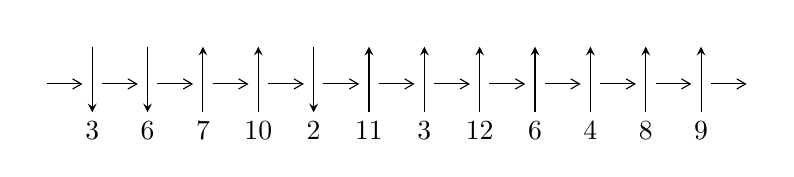
\begin{tikzpicture}[x=20pt, y=17pt]
	% nodes
	\node (C0) at (0, 0) {};
	\node (C1) at (1, 0) {};
	\node (C1U) at (1, +1) {};
	\node (C1D) at (1, -1) {3};

	\node (C2) at (2, 0) {};
	\node (C2U) at (2, +1) {};
	\node (C2D) at (2, -1) {6};

	\node (C3) at (3, 0) {};
	\node (C3U) at (3, +1) {};
	\node (C3D) at (3, -1) {7};

	\node (C4) at (4, 0) {};
	\node (C4U) at (4, +1) {};
	\node (C4D) at (4, -1) {10};

	\node (C5) at (5, 0) {};
	\node (C5U) at (5, +1) {};
	\node (C5D) at (5, -1) {2};

	\node (C6) at (6, 0) {};
	\node (C6U) at (6, +1) {};
	\node (C6D) at (6, -1) {11};

	\node (C7) at (7, 0) {};
	\node (C7U) at (7, +1) {};
	\node (C7D) at (7, -1) {3};

	\node (C8) at (8, 0) {};
	\node (C8U) at (8, +1) {};
	\node (C8D) at (8, -1) {12};

	\node (C9) at (9, 0) {};
	\node (C9U) at (9, +1) {};
	\node (C9D) at (9, -1) {6};

	\node (C10) at (10, 0) {};
	\node (C10U) at (10, +1) {};
	\node (C10D) at (10, -1) {4};

	\node (C11) at (11, 0) {};
	\node (C11U) at (11, +1) {};
	\node (C11D) at (11, -1) {8};

	\node (C12) at (12, 0) {};
	\node (C12U) at (12, +1) {};
	\node (C12D) at (12, -1) {9};
	\node (C13) at (13, 0) {};

	% arrows
	\draw[->,>={angle 60}]
	(C0) edge (C1) (C1) edge (C2) (C2) edge (C3) (C3) edge (C4) (C4) edge (C5) (C5) edge (C6) (C6) edge (C7) (C7) edge (C8) (C8) edge (C9) (C9) edge (C10) (C10) edge (C11) (C11) edge (C12) (C12) edge (C13) ;	\draw[->,>=stealth]
	(C1U) edge (C1D) (C2U) edge (C2D) (C3D) edge (C3U) (C4D) edge (C4U) (C5U) edge (C5D) (C6D) edge (C6U) (C7D) edge (C7U) (C8D) edge (C8U) (C9D) edge (C9U) (C10D) edge (C10U) (C11D) edge (C11U) (C12D) edge (C12U) ;
	\end{tikzpicture} \\
\hhline{~~} \\& 
\textbf{Solving Sequence} \\ \cline{2-2} 
 &
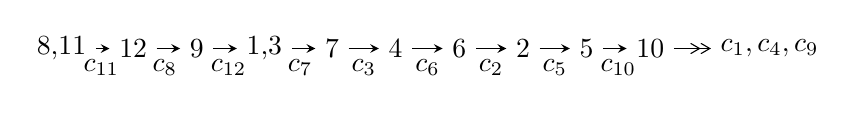
\begin{tikzpicture}[x=23pt, y=7pt]
	% node
	\node (A0) at (-1/8, 0) {8,11};
	\node (A1) at (1, 0) {12};
	\node (A2) at (2, 0) {9};
	\node (A3) at (49/16, 0) {1,3};
	\node (A4) at (33/8, 0) {7};
	\node (A5) at (41/8, 0) {4};
	\node (A6) at (49/8, 0) {6};
	\node (A7) at (57/8, 0) {2};
	\node (A8) at (65/8, 0) {5};
	\node (A9) at (73/8, 0) {10};
	\node (C1) at (1/2, -1) {$c_{11}$};
	\node (C2) at (3/2, -1) {$c_{8}$};
	\node (C3) at (5/2, -1) {$c_{12}$};
	\node (C4) at (29/8, -1) {$c_{7}$};
	\node (C5) at (37/8, -1) {$c_{3}$};
	\node (C6) at (45/8, -1) {$c_{6}$};
	\node (C7) at (53/8, -1) {$c_{2}$};
	\node (C8) at (61/8, -1) {$c_{5}$};
	\node (C9) at (69/8, -1) {$c_{10}$};
	\node (A10) at (11, 0) {$c_{1},c_{4},c_{9}$};

	% edge
	\draw[->,>=stealth]	
	(A0) edge (A1) (A1) edge (A2) (A2) edge (A3) (A3) edge (A4) (A4) edge (A5) (A5) edge (A6) (A6) edge (A7) (A7) edge (A8) (A8) edge (A9) ;
	\draw[->>,>={angle 60}]	
	(A9) edge (A10);
\end{tikzpicture} \\ 

\end{tabular} \\

\footnotetext{
The image of knot diagram is generated by the software ``\textbf{Draw programme}" developed by Andrew Bartholomew(\url{http://www.layer8.co.uk/maths/draw/index.htm\#Running-draw}), where we modified some parts for our purpose(\url{https://github.com/CATsTAILs/LinksPainter}).
}\phantom \\ \newline 
\centering \textbf{Ideals for irreducible components\footnotemark of $X_{\text{par}}$} 
 
\begin{align*}
I^u_{1}&=\langle 
-6.16590\times10^{32} u^{31}+1.46189\times10^{33} u^{30}+\cdots+1.24872\times10^{34} b-5.49780\times10^{33},\\
\phantom{I^u_{1}}&\phantom{= \langle  }-2.37033\times10^{33} u^{31}+4.13166\times10^{33} u^{30}+\cdots+1.24872\times10^{34} a-1.71464\times10^{34},\;u^{32}- u^{31}+\cdots-2 u-1\rangle \\
I^u_{2}&=\langle 
- u^{11}+7 u^9+u^8-18 u^7-5 u^6+21 u^5+7 u^4-11 u^3-2 u^2+b+2 u,\\
\phantom{I^u_{2}}&\phantom{= \langle  }u^{12}-8 u^{10}+25 u^8-40 u^6+u^5+36 u^4-4 u^3-16 u^2+a+4 u+1,\\
\phantom{I^u_{2}}&\phantom{= \langle  }u^{13}-8 u^{11}- u^{10}+25 u^9+6 u^8-39 u^7-12 u^6+32 u^5+9 u^4-13 u^3-2 u^2+2 u+1\rangle \\
\\
\end{align*}
\raggedright * 2 irreducible components of $\dim_{\mathbb{C}}=0$, with total 45 representations.\\
\footnotetext{All coefficients of polynomials are rational numbers. But the coefficients are sometimes approximated in decimal forms when there is not enough margin.}
\newpage
\renewcommand{\arraystretch}{1}
\centering \section*{I. $I^u_{1}= \langle -6.17\times10^{32} u^{31}+1.46\times10^{33} u^{30}+\cdots+1.25\times10^{34} b-5.50\times10^{33},\;-2.37\times10^{33} u^{31}+4.13\times10^{33} u^{30}+\cdots+1.25\times10^{34} a-1.71\times10^{34},\;u^{32}- u^{31}+\cdots-2 u-1 \rangle$}
\flushleft \textbf{(i) Arc colorings}\\
\begin{tabular}{m{7pt} m{180pt} m{7pt} m{180pt} }
\flushright $a_{8}=$&$\begin{pmatrix}0\\u\end{pmatrix}$ \\
\flushright $a_{11}=$&$\begin{pmatrix}1\\0\end{pmatrix}$ \\
\flushright $a_{12}=$&$\begin{pmatrix}1\\- u^2\end{pmatrix}$ \\
\flushright $a_{9}=$&$\begin{pmatrix}u\\- u^3+u\end{pmatrix}$ \\
\flushright $a_{1}=$&$\begin{pmatrix}- u^2+1\\u^4-2 u^2\end{pmatrix}$ \\
\flushright $a_{3}=$&$\begin{pmatrix}0.189821 u^{31}-0.330872 u^{30}+\cdots-5.59851 u+1.37311\\0.0493778 u^{31}-0.117071 u^{30}+\cdots-1.67061 u+0.440274\end{pmatrix}$ \\
\flushright $a_{7}=$&$\begin{pmatrix}0.617113 u^{31}-0.702924 u^{30}+\cdots-2.97277 u-1.56588\\0.255210 u^{31}-0.230274 u^{30}+\cdots+0.144769 u-0.440400\end{pmatrix}$ \\
\flushright $a_{4}=$&$\begin{pmatrix}0.369799 u^{31}-0.365325 u^{30}+\cdots-1.90267 u-0.395284\\0.0271602 u^{31}-0.0677895 u^{30}+\cdots-0.802345 u-0.0663187\end{pmatrix}$ \\
\flushright $a_{6}=$&$\begin{pmatrix}0.361904 u^{31}-0.472651 u^{30}+\cdots-3.11754 u-1.12548\\0.255210 u^{31}-0.230274 u^{30}+\cdots+0.144769 u-0.440400\end{pmatrix}$ \\
\flushright $a_{2}=$&$\begin{pmatrix}0.661372 u^{31}-0.805565 u^{30}+\cdots-5.92579 u-0.0552608\\0.213423 u^{31}-0.264734 u^{30}+\cdots-1.41893 u-0.250047\end{pmatrix}$ \\
\flushright $a_{5}=$&$\begin{pmatrix}-0.276212 u^{31}+0.368159 u^{30}+\cdots+2.60106 u+0.644536\\-0.0127971 u^{31}+0.0681599 u^{30}+\cdots+0.695590 u+0.0648329\end{pmatrix}$ \\
\flushright $a_{10}=$&$\begin{pmatrix}0.209593 u^{31}-0.186992 u^{30}+\cdots-0.405019 u+0.305269\\0.0812154 u^{31}-0.0868146 u^{30}+\cdots+0.236069 u-0.0317778\end{pmatrix}$\\&\end{tabular}
\flushleft \textbf{(ii) Obstruction class $= -1$}\\~\\
\flushleft \textbf{(iii) Cusp Shapes $= 2.64634 u^{31}-2.11189 u^{30}+\cdots+10.8149 u+2.17341$}\\~\\
\newpage\renewcommand{\arraystretch}{1}
\flushleft \textbf{(iv) u-Polynomials at the component}\newline \\
\begin{tabular}{m{50pt}|m{274pt}}
Crossings & \hspace{64pt}u-Polynomials at each crossing \\
\hline $$\begin{aligned}c_{1}\end{aligned}$$&$\begin{aligned}
&u^{32}+50 u^{31}+\cdots+5873 u+169
\end{aligned}$\\
\hline $$\begin{aligned}c_{2},c_{5}\end{aligned}$$&$\begin{aligned}
&u^{32}+2 u^{31}+\cdots+149 u+13
\end{aligned}$\\
\hline $$\begin{aligned}c_{3},c_{7}\end{aligned}$$&$\begin{aligned}
&u^{32}-3 u^{31}+\cdots+6 u+13
\end{aligned}$\\
\hline $$\begin{aligned}c_{4},c_{10}\end{aligned}$$&$\begin{aligned}
&u^{32}+u^{31}+\cdots-12 u-7
\end{aligned}$\\
\hline $$\begin{aligned}c_{6}\end{aligned}$$&$\begin{aligned}
&u^{32}+2 u^{31}+\cdots+2 u-11
\end{aligned}$\\
\hline $$\begin{aligned}c_{8},c_{11},c_{12}\end{aligned}$$&$\begin{aligned}
&u^{32}- u^{31}+\cdots-2 u-1
\end{aligned}$\\
\hline $$\begin{aligned}c_{9}\end{aligned}$$&$\begin{aligned}
&u^{32}+2 u^{31}+\cdots+320 u-448
\end{aligned}$\\
\hline
\end{tabular}\\~\\
\newpage\renewcommand{\arraystretch}{1}
\flushleft \textbf{(v) Riley Polynomials at the component}\newline \\
\begin{tabular}{m{50pt}|m{274pt}}
Crossings & \hspace{64pt}Riley Polynomials at each crossing \\
\hline $$\begin{aligned}c_{1}\end{aligned}$$&$\begin{aligned}
&y^{32}-130 y^{31}+\cdots+545386755 y+28561
\end{aligned}$\\
\hline $$\begin{aligned}c_{2},c_{5}\end{aligned}$$&$\begin{aligned}
&y^{32}-50 y^{31}+\cdots-5873 y+169
\end{aligned}$\\
\hline $$\begin{aligned}c_{3},c_{7}\end{aligned}$$&$\begin{aligned}
&y^{32}+25 y^{31}+\cdots+484 y+169
\end{aligned}$\\
\hline $$\begin{aligned}c_{4},c_{10}\end{aligned}$$&$\begin{aligned}
&y^{32}+47 y^{31}+\cdots+248 y+49
\end{aligned}$\\
\hline $$\begin{aligned}c_{6}\end{aligned}$$&$\begin{aligned}
&y^{32}+4 y^{31}+\cdots+1272 y+121
\end{aligned}$\\
\hline $$\begin{aligned}c_{8},c_{11},c_{12}\end{aligned}$$&$\begin{aligned}
&y^{32}-21 y^{31}+\cdots-10 y+1
\end{aligned}$\\
\hline $$\begin{aligned}c_{9}\end{aligned}$$&$\begin{aligned}
&y^{32}+114 y^{31}+\cdots-5478400 y+200704
\end{aligned}$\\
\hline
\end{tabular}\\~\\
\newpage\flushleft \textbf{(vi) Complex Volumes and Cusp Shapes}
$$\begin{array}{c|c|c}  
\text{Solutions to }I^u_{1}& \I (\text{vol} + \sqrt{-1}CS) & \text{Cusp shape}\\
 \hline 
\begin{aligned}
u &= \phantom{-}0.713734 + 0.634066 I \\
a &= -1.63454 - 0.97058 I \\
b &= -1.090080 + 0.559990 I\end{aligned}
 & -5.38799 + 4.75007 I & \phantom{-}2.65651 - 5.98480 I \\ \hline\begin{aligned}
u &= \phantom{-}0.713734 - 0.634066 I \\
a &= -1.63454 + 0.97058 I \\
b &= -1.090080 - 0.559990 I\end{aligned}
 & -5.38799 - 4.75007 I & \phantom{-}2.65651 + 5.98480 I \\ \hline\begin{aligned}
u &= -0.780100 + 0.713092 I \\
a &= -0.578419 + 0.988520 I \\
b &= -1.43666 - 0.26099 I\end{aligned}
 & -5.66767 + 1.87911 I & \phantom{-}1.97848 + 0.24857 I \\ \hline\begin{aligned}
u &= -0.780100 - 0.713092 I \\
a &= -0.578419 - 0.988520 I \\
b &= -1.43666 + 0.26099 I\end{aligned}
 & -5.66767 - 1.87911 I & \phantom{-}1.97848 - 0.24857 I \\ \hline\begin{aligned}
u &= \phantom{-}0.916172 + 0.567038 I \\
a &= \phantom{-}1.40079 - 1.73118 I \\
b &= \phantom{-}0.403288 + 0.064579 I\end{aligned}
 & -10.08900 + 2.24227 I & -4.41790 - 3.08560 I \\ \hline\begin{aligned}
u &= \phantom{-}0.916172 - 0.567038 I \\
a &= \phantom{-}1.40079 + 1.73118 I \\
b &= \phantom{-}0.403288 - 0.064579 I\end{aligned}
 & -10.08900 - 2.24227 I & -4.41790 + 3.08560 I \\ \hline\begin{aligned}
u &= -0.922337 + 0.681295 I \\
a &= -0.214448 + 0.331259 I \\
b &= \phantom{-}0.63044 - 1.91502 I\end{aligned}
 & -10.84610 - 2.63222 I & -0.52226 + 2.78850 I \\ \hline\begin{aligned}
u &= -0.922337 - 0.681295 I \\
a &= -0.214448 - 0.331259 I \\
b &= \phantom{-}0.63044 + 1.91502 I\end{aligned}
 & -10.84610 + 2.63222 I & -0.52226 - 2.78850 I \\ \hline\begin{aligned}
u &= -1.158300 + 0.287676 I \\
a &= -0.821536 + 1.034540 I \\
b &= -1.035360 - 0.657528 I\end{aligned}
 & \phantom{-}1.13972 - 4.35971 I & \phantom{-}7.21820 + 7.90515 I \\ \hline\begin{aligned}
u &= -1.158300 - 0.287676 I \\
a &= -0.821536 - 1.034540 I \\
b &= -1.035360 + 0.657528 I\end{aligned}
 & \phantom{-}1.13972 + 4.35971 I & \phantom{-}7.21820 - 7.90515 I\\
 \hline 
 \end{array}$$\newpage$$\begin{array}{c|c|c}  
\text{Solutions to }I^u_{1}& \I (\text{vol} + \sqrt{-1}CS) & \text{Cusp shape}\\
 \hline 
\begin{aligned}
u &= -1.040580 + 0.693377 I \\
a &= \phantom{-}0.989786 - 0.571228 I \\
b &= \phantom{-}1.69133 + 0.61668 I\end{aligned}
 & -4.78339 - 7.28882 I & \phantom{-}3.26552 + 6.22364 I \\ \hline\begin{aligned}
u &= -1.040580 - 0.693377 I \\
a &= \phantom{-}0.989786 + 0.571228 I \\
b &= \phantom{-}1.69133 - 0.61668 I\end{aligned}
 & -4.78339 + 7.28882 I & \phantom{-}3.26552 - 6.22364 I \\ \hline\begin{aligned}
u &= \phantom{-}1.220980 + 0.289612 I \\
a &= -0.442917 - 0.682280 I \\
b &= -1.28705 + 0.65034 I\end{aligned}
 & \phantom{-}1.13108 + 1.76995 I & \phantom{-}6.03589 + 2.64881 I \\ \hline\begin{aligned}
u &= \phantom{-}1.220980 - 0.289612 I \\
a &= -0.442917 + 0.682280 I \\
b &= -1.28705 - 0.65034 I\end{aligned}
 & \phantom{-}1.13108 - 1.76995 I & \phantom{-}6.03589 - 2.64881 I \\ \hline\begin{aligned}
u &= \phantom{-}1.110300 + 0.663239 I \\
a &= \phantom{-}0.717757 + 0.805432 I \\
b &= \phantom{-}1.148800 + 0.137989 I\end{aligned}
 & -4.06902 + 0.32626 I & \phantom{-}2.59195 - 0.82777 I \\ \hline\begin{aligned}
u &= \phantom{-}1.110300 - 0.663239 I \\
a &= \phantom{-}0.717757 - 0.805432 I \\
b &= \phantom{-}1.148800 - 0.137989 I\end{aligned}
 & -4.06902 - 0.32626 I & \phantom{-}2.59195 + 0.82777 I \\ \hline\begin{aligned}
u &= \phantom{-}1.44139 + 0.01348 I \\
a &= -0.242696 + 0.203112 I \\
b &= -0.213818 - 0.777820 I\end{aligned}
 & \phantom{-}3.51164 - 2.19651 I & \phantom{-}9.32383 + 3.81660 I \\ \hline\begin{aligned}
u &= \phantom{-}1.44139 - 0.01348 I \\
a &= -0.242696 - 0.203112 I \\
b &= -0.213818 + 0.777820 I\end{aligned}
 & \phantom{-}3.51164 + 2.19651 I & \phantom{-}9.32383 - 3.81660 I \\ \hline\begin{aligned}
u &= \phantom{-}0.08148 + 1.44948 I \\
a &= -1.114080 - 0.266827 I \\
b &= -1.69713 - 0.35935 I\end{aligned}
 & -19.2923 - 4.4522 I & \phantom{-}1.21181 + 2.08819 I \\ \hline\begin{aligned}
u &= \phantom{-}0.08148 - 1.44948 I \\
a &= -1.114080 + 0.266827 I \\
b &= -1.69713 + 0.35935 I\end{aligned}
 & -19.2923 + 4.4522 I & \phantom{-}1.21181 - 2.08819 I\\
 \hline 
 \end{array}$$\newpage$$\begin{array}{c|c|c}  
\text{Solutions to }I^u_{1}& \I (\text{vol} + \sqrt{-1}CS) & \text{Cusp shape}\\
 \hline 
\begin{aligned}
u &= -0.481966 + 0.257396 I \\
a &= \phantom{-}0.87806 + 1.29690 I \\
b &= \phantom{-}0.413129 + 0.311383 I\end{aligned}
 & -1.88542 - 1.30506 I & \phantom{-}1.44155 + 5.20789 I \\ \hline\begin{aligned}
u &= -0.481966 - 0.257396 I \\
a &= \phantom{-}0.87806 - 1.29690 I \\
b &= \phantom{-}0.413129 - 0.311383 I\end{aligned}
 & -1.88542 + 1.30506 I & \phantom{-}1.44155 - 5.20789 I \\ \hline\begin{aligned}
u &= \phantom{-}0.286902 + 0.362783 I \\
a &= \phantom{-}1.65914 + 1.00541 I \\
b &= \phantom{-}1.32318 - 0.60249 I\end{aligned}
 & -1.81266 + 1.48756 I & \phantom{-}1.92285 - 4.94836 I \\ \hline\begin{aligned}
u &= \phantom{-}0.286902 - 0.362783 I \\
a &= \phantom{-}1.65914 - 1.00541 I \\
b &= \phantom{-}1.32318 + 0.60249 I\end{aligned}
 & -1.81266 - 1.48756 I & \phantom{-}1.92285 + 4.94836 I \\ \hline\begin{aligned}
u &= -1.58012\phantom{ +0.000000I} \\
a &= -0.315491\phantom{ +0.000000I} \\
b &= -0.276511\phantom{ +0.000000I}\end{aligned}
 & \phantom{-}7.37313\phantom{ +0.000000I} & \phantom{-}22.2100\phantom{ +0.000000I} \\ \hline\begin{aligned}
u &= \phantom{-}0.409982\phantom{ +0.000000I} \\
a &= \phantom{-}0.726284\phantom{ +0.000000I} \\
b &= -0.225298\phantom{ +0.000000I}\end{aligned}
 & \phantom{-}0.661529\phantom{ +0.000000I} & \phantom{-}15.2090\phantom{ +0.000000I} \\ \hline\begin{aligned}
u &= \phantom{-}1.50304 + 0.73810 I \\
a &= \phantom{-}0.829737 + 0.686971 I \\
b &= \phantom{-}1.59659 - 0.82818 I\end{aligned}
 & -14.9102 + 12.0924 I & \phantom{-0.000000 } 0 \\ \hline\begin{aligned}
u &= \phantom{-}1.50304 - 0.73810 I \\
a &= \phantom{-}0.829737 - 0.686971 I \\
b &= \phantom{-}1.59659 + 0.82818 I\end{aligned}
 & -14.9102 - 12.0924 I & \phantom{-0.000000 } 0 \\ \hline\begin{aligned}
u &= -0.172476 + 0.197273 I \\
a &= \phantom{-}3.03827 - 1.51554 I \\
b &= \phantom{-}0.897886 - 0.510199 I\end{aligned}
 & -1.75865 + 1.40173 I & \phantom{-}0.26124 - 4.99544 I \\ \hline\begin{aligned}
u &= -0.172476 - 0.197273 I \\
a &= \phantom{-}3.03827 + 1.51554 I \\
b &= \phantom{-}0.897886 + 0.510199 I\end{aligned}
 & -1.75865 - 1.40173 I & \phantom{-}0.26124 + 4.99544 I\\
 \hline 
 \end{array}$$\newpage$$\begin{array}{c|c|c}  
\text{Solutions to }I^u_{1}& \I (\text{vol} + \sqrt{-1}CS) & \text{Cusp shape}\\
 \hline 
\begin{aligned}
u &= -1.63318 + 0.69080 I \\
a &= \phantom{-}0.329691 - 0.659740 I \\
b &= \phantom{-}1.406370 + 0.131580 I\end{aligned}
 & -14.0115 - 3.2110 I & \phantom{-0.000000 } 0 \\ \hline\begin{aligned}
u &= -1.63318 - 0.69080 I \\
a &= \phantom{-}0.329691 + 0.659740 I \\
b &= \phantom{-}1.406370 - 0.131580 I\end{aligned}
 & -14.0115 + 3.2110 I & \phantom{-0.000000 } 0\\
 \hline 
 \end{array}$$\newpage\newpage\renewcommand{\arraystretch}{1}
\centering \section*{II. $I^u_{2}= \langle - u^{11}+7 u^9+\cdots+b+2 u,\;u^{12}-8 u^{10}+\cdots+a+1,\;u^{13}-8 u^{11}+\cdots+2 u+1 \rangle$}
\flushleft \textbf{(i) Arc colorings}\\
\begin{tabular}{m{7pt} m{180pt} m{7pt} m{180pt} }
\flushright $a_{8}=$&$\begin{pmatrix}0\\u\end{pmatrix}$ \\
\flushright $a_{11}=$&$\begin{pmatrix}1\\0\end{pmatrix}$ \\
\flushright $a_{12}=$&$\begin{pmatrix}1\\- u^2\end{pmatrix}$ \\
\flushright $a_{9}=$&$\begin{pmatrix}u\\- u^3+u\end{pmatrix}$ \\
\flushright $a_{1}=$&$\begin{pmatrix}- u^2+1\\u^4-2 u^2\end{pmatrix}$ \\
\flushright $a_{3}=$&$\begin{pmatrix}- u^{12}+8 u^{10}-25 u^8+40 u^6- u^5-36 u^4+4 u^3+16 u^2-4 u-1\\u^{11}-7 u^9- u^8+18 u^7+5 u^6-21 u^5-7 u^4+11 u^3+2 u^2-2 u\end{pmatrix}$ \\
\flushright $a_{7}=$&$\begin{pmatrix}- u^{12}+7 u^{10}+\cdots+5 u-3\\- u^{12}+7 u^{10}+\cdots+u-1\end{pmatrix}$ \\
\flushright $a_{4}=$&$\begin{pmatrix}2 u^{12}- u^{11}+\cdots+u+4\\u^{12}-7 u^{10}- u^9+19 u^8+5 u^7-26 u^6-7 u^5+19 u^4+2 u^3-7 u^2+u+1\end{pmatrix}$ \\
\flushright $a_{6}=$&$\begin{pmatrix}u^9-6 u^7+12 u^5-10 u^3+u^2+4 u-2\\- u^{12}+7 u^{10}+\cdots+u-1\end{pmatrix}$ \\
\flushright $a_{2}=$&$\begin{pmatrix}- u^8+6 u^6-12 u^4+8 u^2-1\\u^{11}-7 u^9- u^8+18 u^7+5 u^6-21 u^5-7 u^4+11 u^3+3 u^2-2 u-1\end{pmatrix}$ \\
\flushright $a_{5}=$&$\begin{pmatrix}u^{11}-7 u^9+18 u^7-20 u^5+7 u^3+u^2+2 u-2\\- u^8+5 u^6-8 u^4+5 u^2-1\end{pmatrix}$ \\
\flushright $a_{10}=$&$\begin{pmatrix}2 u^{12}- u^{11}+\cdots+7 u+2\\- u^3+2 u-1\end{pmatrix}$\\&\end{tabular}
\flushleft \textbf{(ii) Obstruction class $= 1$}\\~\\
\flushleft \textbf{(iii) Cusp Shapes $= -2 u^{12}-2 u^{11}+16 u^{10}+15 u^9-47 u^8-42 u^7+64 u^6+54 u^5-46 u^4-29 u^3+17 u^2+2 u+5$}\\~\\
\newpage\renewcommand{\arraystretch}{1}
\flushleft \textbf{(iv) u-Polynomials at the component}\newline \\
\begin{tabular}{m{50pt}|m{274pt}}
Crossings & \hspace{64pt}u-Polynomials at each crossing \\
\hline $$\begin{aligned}c_{1}\end{aligned}$$&$\begin{aligned}
&u^{13}-13 u^{12}+\cdots+7 u-1
\end{aligned}$\\
\hline $$\begin{aligned}c_{2}\end{aligned}$$&$\begin{aligned}
&u^{13}+3 u^{12}+\cdots-3 u-1
\end{aligned}$\\
\hline $$\begin{aligned}c_{3}\end{aligned}$$&$\begin{aligned}
&u^{13}+3 u^{11}+\cdots+6 u-1
\end{aligned}$\\
\hline $$\begin{aligned}c_{4}\end{aligned}$$&$\begin{aligned}
&u^{13}+8 u^{11}+24 u^9+u^8+33 u^7+4 u^6+20 u^5+5 u^4+5 u^3+u^2+2 u-1
\end{aligned}$\\
\hline $$\begin{aligned}c_{5}\end{aligned}$$&$\begin{aligned}
&u^{13}-3 u^{12}+\cdots-3 u+1
\end{aligned}$\\
\hline $$\begin{aligned}c_{6}\end{aligned}$$&$\begin{aligned}
&u^{13}+u^{12}- u^{11}- u^{10}-2 u^7-9 u^6-2 u^5-7 u^4-3 u^3-3 u^2-1
\end{aligned}$\\
\hline $$\begin{aligned}c_{7}\end{aligned}$$&$\begin{aligned}
&u^{13}+3 u^{11}+\cdots+6 u+1
\end{aligned}$\\
\hline $$\begin{aligned}c_{8}\end{aligned}$$&$\begin{aligned}
&u^{13}-8 u^{11}+\cdots+2 u-1
\end{aligned}$\\
\hline $$\begin{aligned}c_{9}\end{aligned}$$&$\begin{aligned}
&u^{13}+u^{12}+\cdots- u+1
\end{aligned}$\\
\hline $$\begin{aligned}c_{10}\end{aligned}$$&$\begin{aligned}
&u^{13}+8 u^{11}+24 u^9- u^8+33 u^7-4 u^6+20 u^5-5 u^4+5 u^3- u^2+2 u+1
\end{aligned}$\\
\hline $$\begin{aligned}c_{11},c_{12}\end{aligned}$$&$\begin{aligned}
&u^{13}-8 u^{11}+\cdots+2 u+1
\end{aligned}$\\
\hline
\end{tabular}\\~\\
\newpage\renewcommand{\arraystretch}{1}
\flushleft \textbf{(v) Riley Polynomials at the component}\newline \\
\begin{tabular}{m{50pt}|m{274pt}}
Crossings & \hspace{64pt}Riley Polynomials at each crossing \\
\hline $$\begin{aligned}c_{1}\end{aligned}$$&$\begin{aligned}
&y^{13}-21 y^{12}+\cdots-21 y-1
\end{aligned}$\\
\hline $$\begin{aligned}c_{2},c_{5}\end{aligned}$$&$\begin{aligned}
&y^{13}-13 y^{12}+\cdots+7 y-1
\end{aligned}$\\
\hline $$\begin{aligned}c_{3},c_{7}\end{aligned}$$&$\begin{aligned}
&y^{13}+6 y^{12}+\cdots+22 y-1
\end{aligned}$\\
\hline $$\begin{aligned}c_{4},c_{10}\end{aligned}$$&$\begin{aligned}
&y^{13}+16 y^{12}+\cdots+6 y-1
\end{aligned}$\\
\hline $$\begin{aligned}c_{6}\end{aligned}$$&$\begin{aligned}
&y^{13}-3 y^{12}+\cdots-6 y-1
\end{aligned}$\\
\hline $$\begin{aligned}c_{8},c_{11},c_{12}\end{aligned}$$&$\begin{aligned}
&y^{13}-16 y^{12}+\cdots+8 y-1
\end{aligned}$\\
\hline $$\begin{aligned}c_{9}\end{aligned}$$&$\begin{aligned}
&y^{13}+23 y^{12}+\cdots+15 y-1
\end{aligned}$\\
\hline
\end{tabular}\\~\\
\newpage\flushleft \textbf{(vi) Complex Volumes and Cusp Shapes}
$$\begin{array}{c|c|c}  
\text{Solutions to }I^u_{2}& \I (\text{vol} + \sqrt{-1}CS) & \text{Cusp shape}\\
 \hline 
\begin{aligned}
u &= -1.001170 + 0.552293 I \\
a &= \phantom{-}0.875628 + 0.971745 I \\
b &= \phantom{-}0.230247 - 0.841237 I\end{aligned}
 & -9.35275 - 2.09354 I & \phantom{-}7.20188 + 0.46928 I \\ \hline\begin{aligned}
u &= -1.001170 - 0.552293 I \\
a &= \phantom{-}0.875628 - 0.971745 I \\
b &= \phantom{-}0.230247 + 0.841237 I\end{aligned}
 & -9.35275 + 2.09354 I & \phantom{-}7.20188 - 0.46928 I \\ \hline\begin{aligned}
u &= \phantom{-}1.229660 + 0.182594 I \\
a &= -0.338886 - 0.829343 I \\
b &= -1.11117 + 1.04233 I\end{aligned}
 & \phantom{-}0.99221 + 2.74184 I & \phantom{-}3.93696 - 4.65266 I \\ \hline\begin{aligned}
u &= \phantom{-}1.229660 - 0.182594 I \\
a &= -0.338886 + 0.829343 I \\
b &= -1.11117 - 1.04233 I\end{aligned}
 & \phantom{-}0.99221 - 2.74184 I & \phantom{-}3.93696 + 4.65266 I \\ \hline\begin{aligned}
u &= -1.298440 + 0.119369 I \\
a &= -0.766018 + 1.016630 I \\
b &= -1.227350 - 0.566412 I\end{aligned}
 & -1.21383 - 4.55409 I & \phantom{-}3.28508 + 3.98345 I \\ \hline\begin{aligned}
u &= -1.298440 - 0.119369 I \\
a &= -0.766018 - 1.016630 I \\
b &= -1.227350 + 0.566412 I\end{aligned}
 & -1.21383 + 4.55409 I & \phantom{-}3.28508 - 3.98345 I \\ \hline\begin{aligned}
u &= \phantom{-}0.572766 + 0.333551 I \\
a &= \phantom{-}0.953439 + 0.550346 I \\
b &= \phantom{-}1.031350 + 0.503157 I\end{aligned}
 & -1.38489 - 0.74935 I & \phantom{-}5.96891 - 3.49027 I \\ \hline\begin{aligned}
u &= \phantom{-}0.572766 - 0.333551 I \\
a &= \phantom{-}0.953439 - 0.550346 I \\
b &= \phantom{-}1.031350 - 0.503157 I\end{aligned}
 & -1.38489 + 0.74935 I & \phantom{-}5.96891 + 3.49027 I \\ \hline\begin{aligned}
u &= -0.294410 + 0.263773 I \\
a &= \phantom{-}1.38207 - 3.00576 I \\
b &= \phantom{-}0.992614 - 0.156850 I\end{aligned}
 & -4.69980 + 3.16875 I & \phantom{-}5.12846 - 3.30315 I \\ \hline\begin{aligned}
u &= -0.294410 - 0.263773 I \\
a &= \phantom{-}1.38207 + 3.00576 I \\
b &= \phantom{-}0.992614 + 0.156850 I\end{aligned}
 & -4.69980 - 3.16875 I & \phantom{-}5.12846 + 3.30315 I\\
 \hline 
 \end{array}$$\newpage$$\begin{array}{c|c|c}  
\text{Solutions to }I^u_{2}& \I (\text{vol} + \sqrt{-1}CS) & \text{Cusp shape}\\
 \hline 
\begin{aligned}
u &= \phantom{-}1.60888 + 0.07753 I \\
a &= -0.048946 - 0.541592 I \\
b &= -0.616598 + 0.097202 I\end{aligned}
 & \phantom{-}2.26514 - 1.76839 I & \phantom{-}2.54626 + 1.07577 I \\ \hline\begin{aligned}
u &= \phantom{-}1.60888 - 0.07753 I \\
a &= -0.048946 + 0.541592 I \\
b &= -0.616598 - 0.097202 I\end{aligned}
 & \phantom{-}2.26514 + 1.76839 I & \phantom{-}2.54626 - 1.07577 I \\ \hline\begin{aligned}
u &= -1.63455\phantom{ +0.000000I} \\
a &= -0.114567\phantom{ +0.000000I} \\
b &= -0.598176\phantom{ +0.000000I}\end{aligned}
 & \phantom{-}7.04862\phantom{ +0.000000I} & -3.13510\phantom{ +0.000000I}\\
 \hline 
 \end{array}$$\newpage
\newpage\renewcommand{\arraystretch}{1}
\centering \section*{ III. u-Polynomials}
\begin{tabular}{m{50pt}|m{274pt}}
Crossings & \hspace{64pt}u-Polynomials at each crossing \\
\hline $$\begin{aligned}c_{1}\end{aligned}$$&$\begin{aligned}
&(u^{13}-13 u^{12}+\cdots+7 u-1)(u^{32}+50 u^{31}+\cdots+5873 u+169)
\end{aligned}$\\
\hline $$\begin{aligned}c_{2}\end{aligned}$$&$\begin{aligned}
&(u^{13}+3 u^{12}+\cdots-3 u-1)(u^{32}+2 u^{31}+\cdots+149 u+13)
\end{aligned}$\\
\hline $$\begin{aligned}c_{3}\end{aligned}$$&$\begin{aligned}
&(u^{13}+3 u^{11}+\cdots+6 u-1)(u^{32}-3 u^{31}+\cdots+6 u+13)
\end{aligned}$\\
\hline $$\begin{aligned}c_{4}\end{aligned}$$&$\begin{aligned}
&(u^{13}+8 u^{11}+24 u^9+u^8+33 u^7+4 u^6+20 u^5+5 u^4+5 u^3+u^2+2 u-1)\\
&\cdot(u^{32}+u^{31}+\cdots-12 u-7)
\end{aligned}$\\
\hline $$\begin{aligned}c_{5}\end{aligned}$$&$\begin{aligned}
&(u^{13}-3 u^{12}+\cdots-3 u+1)(u^{32}+2 u^{31}+\cdots+149 u+13)
\end{aligned}$\\
\hline $$\begin{aligned}c_{6}\end{aligned}$$&$\begin{aligned}
&(u^{13}+u^{12}- u^{11}- u^{10}-2 u^7-9 u^6-2 u^5-7 u^4-3 u^3-3 u^2-1)\\
&\cdot(u^{32}+2 u^{31}+\cdots+2 u-11)
\end{aligned}$\\
\hline $$\begin{aligned}c_{7}\end{aligned}$$&$\begin{aligned}
&(u^{13}+3 u^{11}+\cdots+6 u+1)(u^{32}-3 u^{31}+\cdots+6 u+13)
\end{aligned}$\\
\hline $$\begin{aligned}c_{8}\end{aligned}$$&$\begin{aligned}
&(u^{13}-8 u^{11}+\cdots+2 u-1)(u^{32}- u^{31}+\cdots-2 u-1)
\end{aligned}$\\
\hline $$\begin{aligned}c_{9}\end{aligned}$$&$\begin{aligned}
&(u^{13}+u^{12}+\cdots- u+1)(u^{32}+2 u^{31}+\cdots+320 u-448)
\end{aligned}$\\
\hline $$\begin{aligned}c_{10}\end{aligned}$$&$\begin{aligned}
&(u^{13}+8 u^{11}+24 u^9- u^8+33 u^7-4 u^6+20 u^5-5 u^4+5 u^3- u^2+2 u+1)\\
&\cdot(u^{32}+u^{31}+\cdots-12 u-7)
\end{aligned}$\\
\hline $$\begin{aligned}c_{11},c_{12}\end{aligned}$$&$\begin{aligned}
&(u^{13}-8 u^{11}+\cdots+2 u+1)(u^{32}- u^{31}+\cdots-2 u-1)
\end{aligned}$\\
\hline
\end{tabular}\newpage\renewcommand{\arraystretch}{1}
\centering \section*{ IV. Riley Polynomials}
\begin{tabular}{m{50pt}|m{274pt}}
Crossings & \hspace{64pt}Riley Polynomials at each crossing \\
\hline $$\begin{aligned}c_{1}\end{aligned}$$&$\begin{aligned}
&(y^{13}-21 y^{12}+\cdots-21 y-1)\\
&\cdot(y^{32}-130 y^{31}+\cdots+545386755 y+28561)
\end{aligned}$\\
\hline $$\begin{aligned}c_{2},c_{5}\end{aligned}$$&$\begin{aligned}
&(y^{13}-13 y^{12}+\cdots+7 y-1)(y^{32}-50 y^{31}+\cdots-5873 y+169)
\end{aligned}$\\
\hline $$\begin{aligned}c_{3},c_{7}\end{aligned}$$&$\begin{aligned}
&(y^{13}+6 y^{12}+\cdots+22 y-1)(y^{32}+25 y^{31}+\cdots+484 y+169)
\end{aligned}$\\
\hline $$\begin{aligned}c_{4},c_{10}\end{aligned}$$&$\begin{aligned}
&(y^{13}+16 y^{12}+\cdots+6 y-1)(y^{32}+47 y^{31}+\cdots+248 y+49)
\end{aligned}$\\
\hline $$\begin{aligned}c_{6}\end{aligned}$$&$\begin{aligned}
&(y^{13}-3 y^{12}+\cdots-6 y-1)(y^{32}+4 y^{31}+\cdots+1272 y+121)
\end{aligned}$\\
\hline $$\begin{aligned}c_{8},c_{11},c_{12}\end{aligned}$$&$\begin{aligned}
&(y^{13}-16 y^{12}+\cdots+8 y-1)(y^{32}-21 y^{31}+\cdots-10 y+1)
\end{aligned}$\\
\hline $$\begin{aligned}c_{9}\end{aligned}$$&$\begin{aligned}
&(y^{13}+23 y^{12}+\cdots+15 y-1)\\
&\cdot(y^{32}+114 y^{31}+\cdots-5478400 y+200704)
\end{aligned}$\\
\hline
\end{tabular}
\vskip 2pc
\end{document}